\begin{figure}
 \centering
 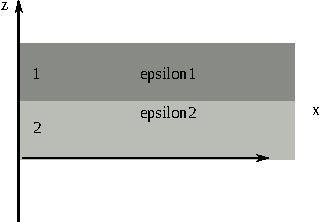
\includegraphics{existence/figures/singlelayerinterfacegeo.pdf}
 \caption{Geometry and coordinate system for the single interface system.}
\end{figure}
With plane wave solutions in hand, boundary conditions consistent with a
single interface can be imposed.
At a planar interface, it is convenient to restrict the problem to TM
polarization in two dimensions; in this case the $x$-$z$ plane as shown in
\Figure{fig:singleinterfacegeo}. Since $\mathbf{k}=(k_x,0,k_z)$,
$\mathbf{r}\cdot\mathbf{k}=k_x x + k_z z$ and $\mathbf{E}_0 = (E_x, 0,
E_z)$, the electric field can be written 
\begin{align}
\mathbf{E} ( \mathbf{r}, t ) &= \mathbf{E}_0\, \me^{\mi (\mathbf{k}
\cdot \mathbf{r} - \omega t )}\\
\mathbf{E}(x,z,t)&=\begin{pmatrix}
E_x\\ 0\\ E_z
\end{pmatrix}
\, \me^{\mi(k_{x,i}x+k_{z,i}z-\omega t)}
\label{eqn:planewavexz}
\end{align}
The magnetic field propagates in the same direction with the
same $\mathbf{k}$-vector components, but the direction
$\mathbf{H}$ must be orthogonal to $\mathbf{E}$ by
\Equation{eqn:faradayslaw}
\begin{align}
\mathbf{H} ( \mathbf{r}, t ) &= \mathbf{H}_0\, \me^{\mi (\mathbf{k}
\cdot \mathbf{r} - \omega t )}\\
\mathbf{H}(x,z,t)&=\begin{pmatrix}
0\\ H_y\\ 0
\end{pmatrix}
\, \me^{\mi(k_{x,i}x+k_{z,i}z-\omega t)}
\end{align}
At the interface there are two values for the (complex) permittivity,
$\epsilon_1$ and $\epsilon_2$.  Consequently
there are two sets of plane wave solutions
\begin{align}
\left.\begin{aligned}
\mathbf{H}_1(x,z,t) &=
\begin{pmatrix}
0\\
H_{y,1}\\
0
\end{pmatrix} \me^{\mi(k_{x,1}x+k_{z,1}z-\omega t)}\\
\mathbf{E}_1(x,z,t) &=
\begin{pmatrix}
E_{x,1}\\
0\\
E_{z,1}\\
\end{pmatrix} \me^{\mi(k_{x,1}x+k_{z,1}z-\omega t)}
\end{aligned}
\right\}& \quad \epsilon_1\label{eqn:planewavedielectric}\\
\left.\begin{aligned}
\mathbf{H}_2(x,z,t) &=
\begin{pmatrix}
0\\
H_{y,2}\\
0
\end{pmatrix}
\me^{\mi(k_{x,2}x+k_{z,2}z-\omega t)}\\
\mathbf{E}_2(x,z,t) &=
\begin{pmatrix}
E_{x,2}\\
0\\
E_{z,2}\\
\end{pmatrix}
\me^{\mi(k_{x,2}x+k_{z,2}z-\omega t)}
\end{aligned} 
\right\}&\quad \epsilon_2
\label{eqn:planewavemetal}
\end{align}
where the subscript designates which material the wave equation refers to.
(e.g. $\mathbf{E}_1$ is the electric field in $\epsilon_1$, $\mathbf{H}_2$
the magnetic field in the $\epsilon_2$, etc.)
Continuity of \Equation{eqn:planewavedielectric} and
\ref{eqn:planewavemetal} at this interface requires that
\begin{align}
E_{x,2}&=E_{x,1}\\
H_{y,2}&=H_{y,1}\\
\epsilon_2 E_{z,2}&=\epsilon_1 E_{z,1}
\end{align}
Applying Ampere's law (\Equation{eqn:ampereslaw}) to the field on the
each boundary gives
\begin{align}
\nabla \times \mathbf{H}_i &= \epsilon_i \frac{\partial \mathbf{E}_i}{\partial t}\\
\begin{pmatrix}
\frac{\partial H_{z,i}}{\partial y} - \frac{\partial H_{y,i}}{\partial z}\\
\frac{\partial H_{x,i}}{\partial y} - \frac{\partial H_{z,i}}{\partial z}\\
\frac{\partial H_{y,i}}{\partial y} - \frac{\partial H_{x,i}}{\partial z}
\end{pmatrix}
&= \begin{pmatrix}
-\mi k_{z,i} H_{y,i}\\
0\\
\mi k_{x,i} H_{y,i}
\end{pmatrix}
\\
&= \begin{pmatrix}
-\mi \omega \epsilon_i E_{x,i}\\
0\\
-\mi \omega \epsilon_i E_{z,i}
\end{pmatrix}
\label{eqn:vectordisp}
\end{align}
where $\mathbf{E}_i$, $\mathbf{H}_i$, $i=1,2$ represent the field in either the
$\epsilon_1$ or $\epsilon_2$.  The vector components of
\Equation{eqn:vectordisp} are therefore related 
\begin{align}
-\mi k_{z,i} H_{y,i} &= -\mi \omega \epsilon_i E_{x,i}\\
k_{z,1} H_{y,1} &= \omega \epsilon_1 E_{x,1}\\
k_{z,2} H_{y,2} &= \omega \epsilon_2 E_{x,2}
\label{eqn:spderivsteptwo}
\end{align}
Since the components of both $\mathbf{E}_i$ and $\mathbf{H}_i$ are
parallel to the interface, $E_{x,i}$ and $H_{y,i}$ are also
continuous. By substitution of $E_{x,i}$, \Equation{eqn:spderivsteptwo} becomes
\begin{align}
\frac{k_{z,1}}{\epsilon_1}H_{y,1}&=\frac{k_{z,2}}{\epsilon_2}H_{y,2}\\ 
\Aboxed{
\frac{k_{z,1}}{\epsilon_1}&=\frac{k_{z,2}}{\epsilon_2} 
}
\label{eqn:sprcondition}
\end{align}
This is the surface plasmon resonance condition.  Note an important aspect
of \Equation{eqn:sprcondition}.  Due to the way we have defined our
geometry, $k_{z,1}$ must be postive and $k_{z,2}$ negative.  For
\Equation{eqn:sprcondition} to hold, this implies that the real part of
$\epsilon_1$ and $\epsilon_2$ are opposite in sign.  For materials we know
exist, this is fulfilled if $\epsilon_1$ is a dielectric and $\epsilon_2$
is a metal.
% Maybe add here how it won't work with TE polarization
